\chapter{Project Description}
\setlength{\parindent}{15pt}
\label{ch:proj_desc}

This chapter will elaborate on the objective of the project and the mission of the product. The functions that the product needs to perform will be evaluated.  

\section{Mission Description}
\label{sec:miss_desc}
The Hybrid UAV is designed in order to have a wide range of missions and applications. The five identified main markets are listed in this section.
\nomenclature{UAV}{Unmanned Aerial Vehicle}

\begin{enumerate}
\item	Search and rescue and support to disaster relief operations.
\item	Precision agriculture by monitoring of cattle and crops.
\item  Transportation of parcels at sea and on land.
\item Inspection of extensive industrial assets and infrastructures such as railways, high-tension power lines, pipelines, wind farms, etc.
\item Transportation of organs for transplants.
\end{enumerate}


\section{Functional Analysis}
\label{ch:func_anal}
\setlength{\parindent}{15pt}

In this section the functions of the UAV are analysed by means of illustrating the functional flow diagram and functional breakdown structure. 

\subsection{Functional Flow Diagram}

In this section, the functional flow diagram of the project is illustrated and explained. The functional flow diagram can be found in \autoref{fig:FuncFlow}. The top-level flow of each mission is illustrated on top of the figure. Each rectangle corresponds to a specific function to be performed and can be further elaborated on in a function-branch indicated by REF. Depending on the statement, a GO (G) or NO GO ($\overline{G}$) may follow the function. 

\begin{figure}[htb]
\centering
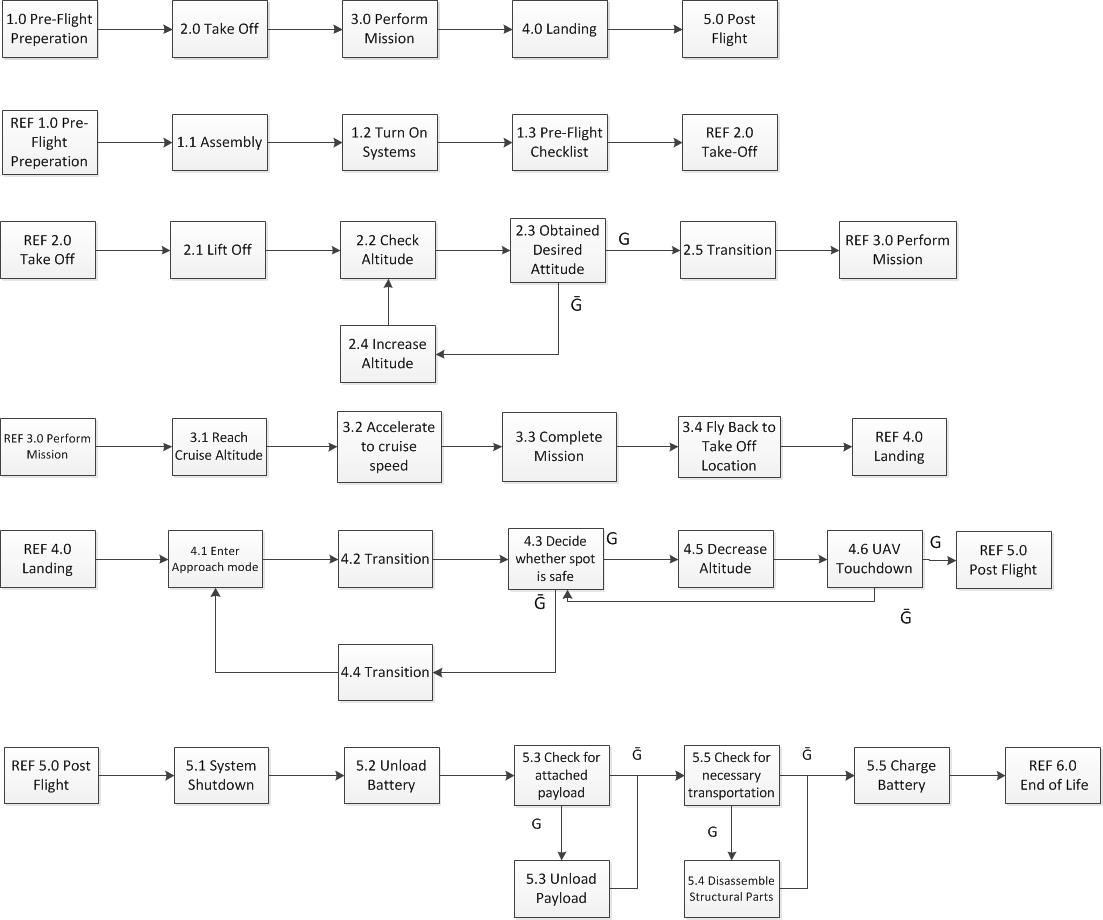
\includegraphics[width=\textwidth]{./ProjectDescription/Figures/ALL}
\caption{Functional flow diagram}
\label{fig:FuncFlow}
\end{figure}

The functional flow diagram is applicable on all missions stated in \autoref{sec:miss_desc}. First, the pre-flight preparations are carried out. Secondly, take-off and transition take place. Then, The mission will be performed. Followed by the transition and landing. Finally, the post-flight procedures can be carried out. Each mission phase consists of flying at cruise altitude and cruise speed towards the mission destination. However, function 3.3 Complete Mission is a mission specific function block. Depending on what mission the UAV has to fly, the UAV will have to perform different functions such as hovering, loitering, dropping of packages, ...

\subsection{Functional Breakdown Structure}

\autoref{fig:FBS} shows the functional breakdown diagram where all top-level functions combined make the UAV system operative. The general structure was adapted from an example air transport mission \cite{SE_notes_2006}. The basic function of performing air transport is separated from performing missions and operate under various conditions. "Perform air transport" translates the pre-flight operations, take-off preparations, flight operations and post-landing operation mission phases into functions. Since the flight operations are both important and extensive, they have a separate break-down in \autoref{fig:FBS-FlightOps}. 

It was identified previously that the main mission profiles are monitoring, transport between bases, transport with aerial drop-off and combinations of them. Hence, there have to be functions that enable those operations, e.g. the ability to follow predefined way points. The conditions under which these missions can be performed can be grouped into: normal operating conditions, under which the UAV can achieve its maximum performance, abnormal conditions, where limited flight operations are still possible, and emergency situations, in which safety for the UAV and its environment has to be ensured. 


\begin{figure}[htb]
\centering
2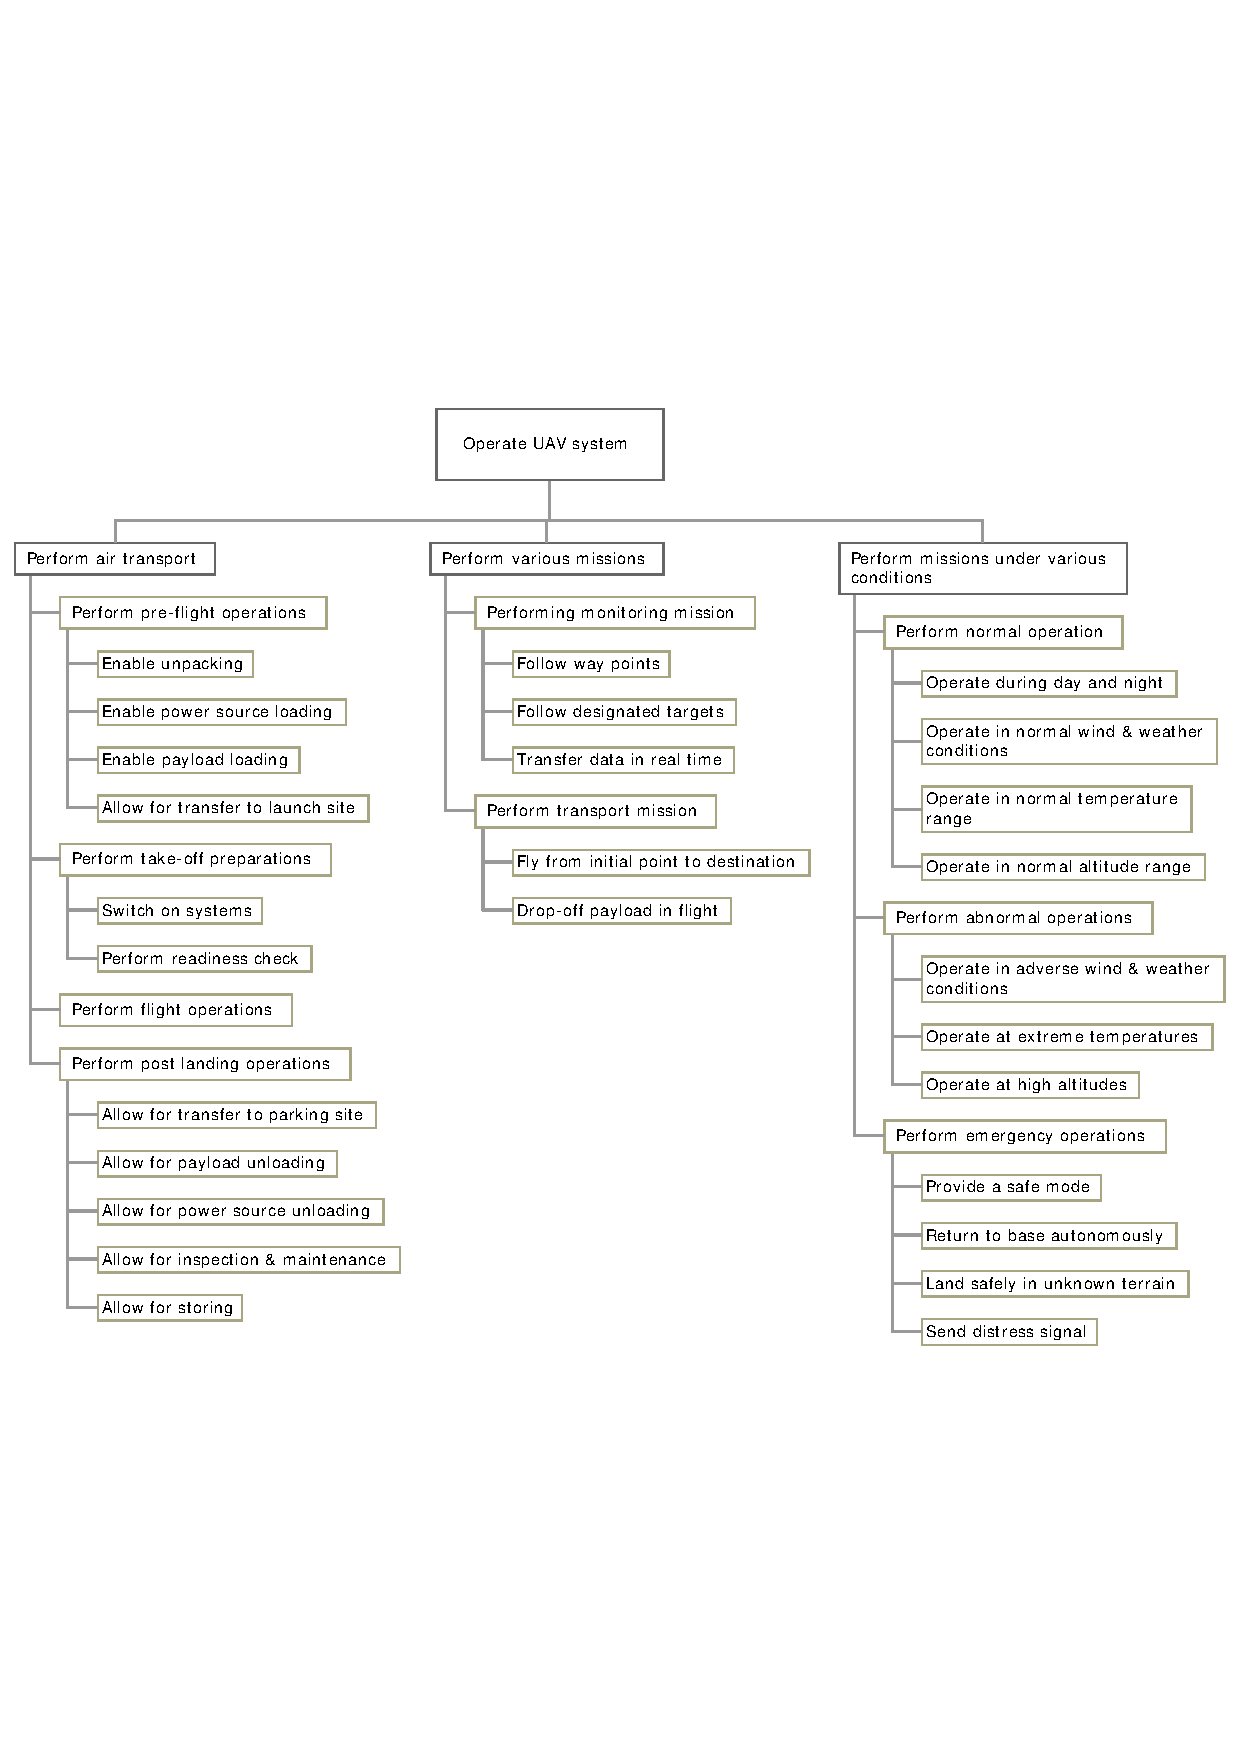
\includegraphics[width=\textwidth]{./ProjectDescription/Figures/FBS}
\caption{Functional breakdown structure}
\label{fig:FBS}
\end{figure}

\begin{figure}[htb]
\centering
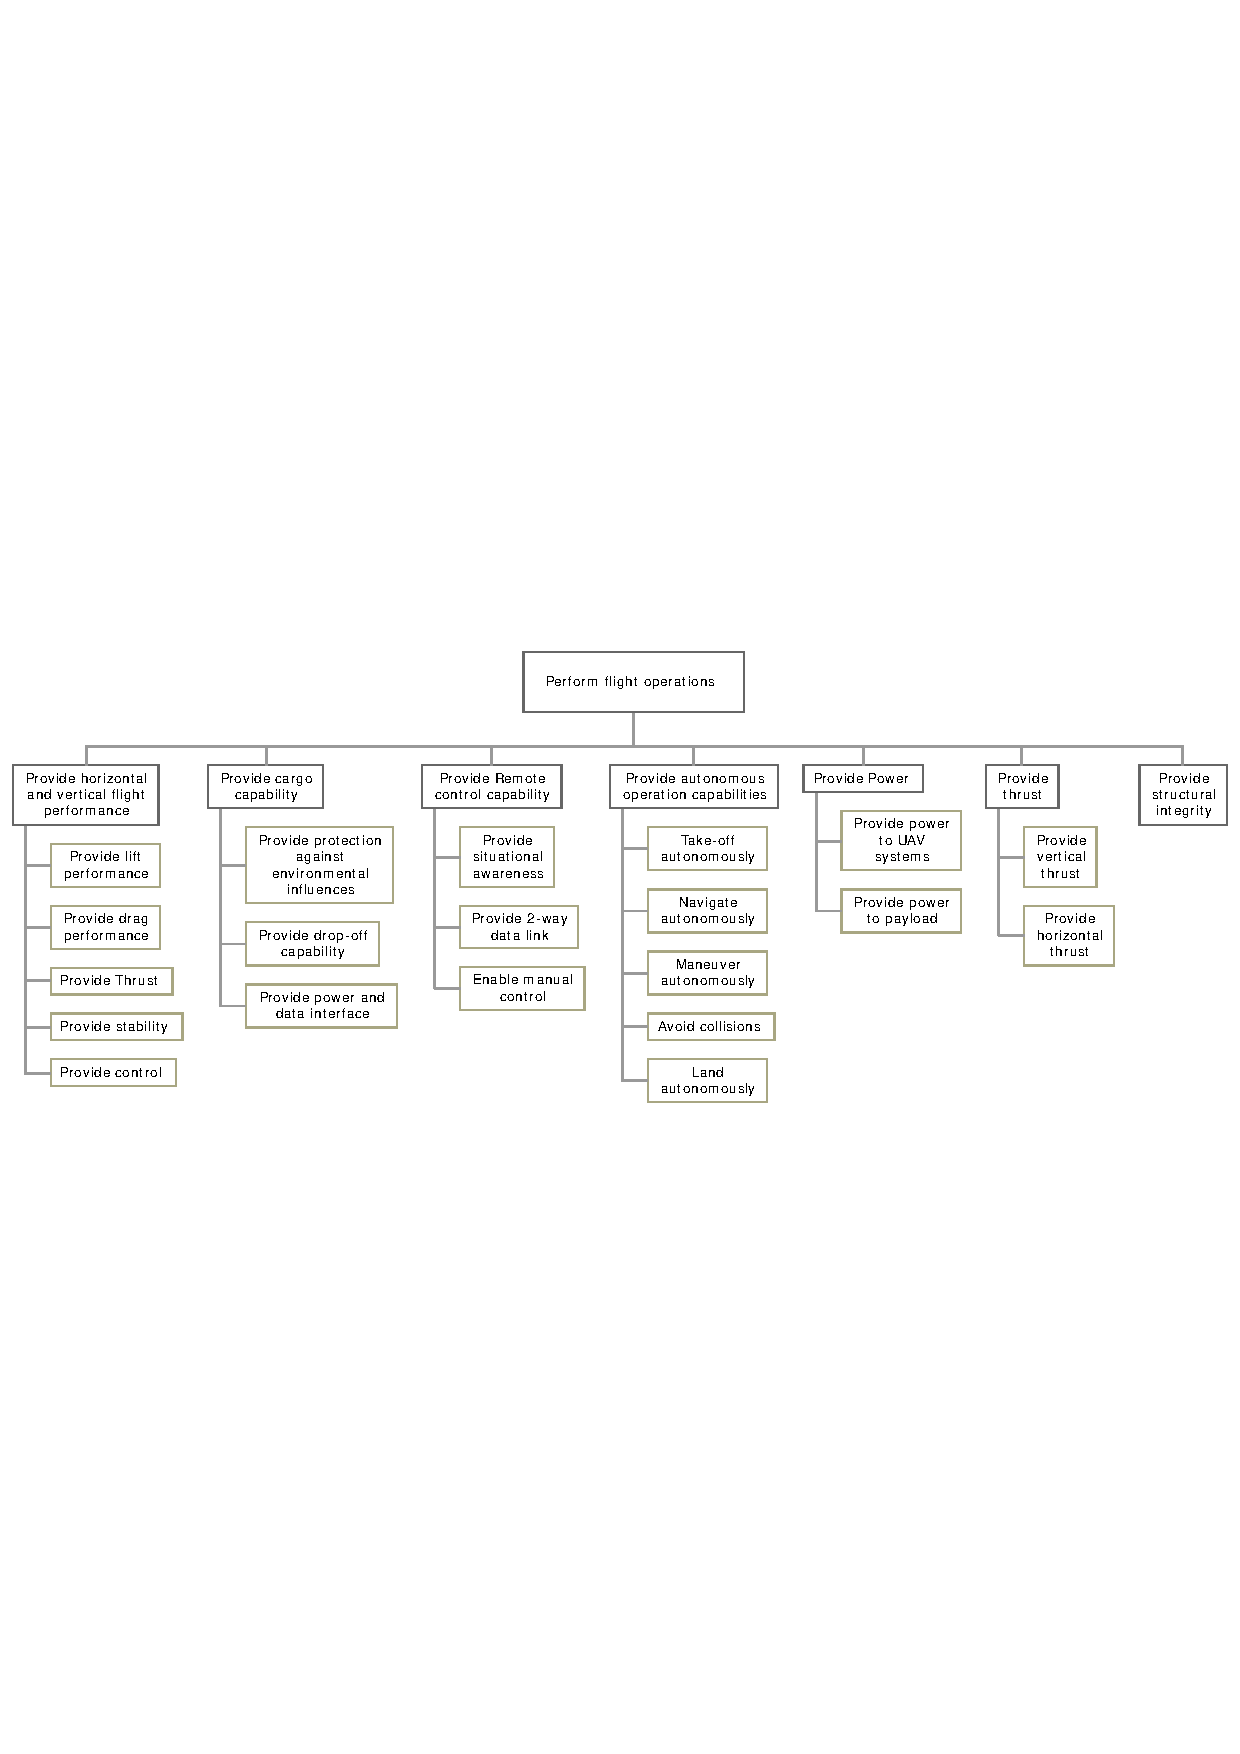
\includegraphics[width=\textwidth]{./ProjectDescription/Figures/FBS-FlightOps}
\caption{Perform flight operations function}
\label{fig:FBS-FlightOps}
\end{figure}


